\documentclass[10pt,xcolor=pdflatex]{beamer}
\usepackage{newcent}
\usepackage[utf8]{inputenc}
\usepackage[czech]{babel}
\usepackage{hyperref}
\usepackage{textpos}
\usepackage{multicol}
\usepackage{tikz}
\usepackage{fancyvrb}
\usepackage{color}
\usepackage{subfig}
\usepackage{geometry}
\usepackage{graphicx}
\usepackage{epstopdf}
\usepackage{lmodern}
\usepackage{todonotes}

\epstopdfDeclareGraphicsRule{.gif}{png}{.png}{convert gif:#1 png:\OutputFile}
\AppendGraphicsExtensions{.gif}
\usetheme{FIT}

\def\uv#1{\quotedblbase#1\textquotedblleft}%

%%%%%%%%%%%%%%%%%%%%%%%%%%%%%%%%%%%%%%%%%%%%%%%%%%%%%%%%%%%%%%%%%%
\title[GJA 5]{PrimeFaces}

\author[]{Jaroslav Dytrych}

\institute[]{Faculty of Information Technology
Brno University of Technology \\
Bo\v{z}et\v{e}chova 1/2. 612 66 Brno - Kr\'alovo Pole\\
dytrych@fit.vutbr.cz}

\date{24 October 2023}
%\date{\today}
%\date{} % bez data

%%%%%%%%%%%%%%%%%%%%%%%%%%%%%%%%%%%%%%%%%%%%%%%%%%%%%%%%%%%%%%%%%%

\begin{document}

\makeatletter
\g@addto@macro{\UrlBreaks}{\UrlOrds}
\makeatother

\frame[plain]{\titlepage}

\bluepage{PrimeFaces}

\begin{frame}\frametitle{Introduction}
  \begin{itemize}
    \item JSF doesn't provide rich set of components
	  \begin{itemize}
		\item It is left for $3^{rd}$ party libraries
	  \end{itemize}
    \item PrimeFaces
      \begin{itemize}
    	\item rich set of components
		\item uses JQuery library for custom components
		\item AJAX support (based on JSF 2.0)
		\item push support via Atmosphere framework (WebSocket/Comet)
		  \begin{itemize}
		      \item In 7.0 Push has been removed. Please use the JSF 2.3 socket or OmniFaces now.
		  \end{itemize}
		\item one-jar library, no configuration nor dependencies
		\item lots of built-in themes, visual theme designer tool
		  \begin{itemize}
		      \item Old versions ThemeRoller \url{https://jqueryui.com/themeroller/}
		      \item Theme Designer \url{https://www.primefaces.org/designer-jsf/}
		  \end{itemize}
		\item extensive documentation
		\item XHTML facelets on client combined with Java on the server side
      \end{itemize}
  \end{itemize}
\begin{tikzpicture}[remember picture,overlay]
    \node[xshift=-0.6cm,yshift=-1.3cm] at (current page.north east){%
    
\includegraphics[width=1cm]{img/pozor}};
\end{tikzpicture}
\end{frame}


\begin{frame}\frametitle{Content}
  \begin{itemize}
    \item PrimeFaces
      \begin{itemize}
    	\item Theming concept
		\item Inputs and selects
		\item Client side validations
		\item Panels
		\item Data iteration components
		\item Menus
		\item Dialog framework
		\item Working with files and images
		\item Drag \& Drop
		\item Charts
		\item Push
		\item RequestContext (\texttt{PrimeFaces.current()})
      \end{itemize}
  \end{itemize}
\end{frame}


\begin{frame}[containsverbatim]\frametitle{Theming concept}
  \begin{itemize}
    \item Themes
	  \begin{itemize}
		\item 10 Built-In Themes
		\item 18 Premium Themes
		\item 38 Community Themes
	  \end{itemize}
    \item Configuration (\texttt{web.xml})
    \item[] \begin{verbatim}
<context-param>
    <param-name>primefaces.THEME</param-name>
    <param-value>aristo</param-value>
</context-param>
\end{verbatim} 
    \item May be dynamic
    \begin{footnotesize}
      \item[] \begin{verbatim}
<context-param>
    <param-name>primefaces.THEME</param-name>
    <param-value>#{loggedInUser.preferences.theme}</param-value>
</context-param>		
		\end{verbatim}
    \end{footnotesize}   
  \end{itemize}
\begin{tikzpicture}[remember picture,overlay]
    \node[xshift=-0.6cm,yshift=-1.3cm] at (current page.north east){%
    
\includegraphics[width=1cm]{img/oko}};
\end{tikzpicture}
\end{frame}


\begin{frame}[containsverbatim]\frametitle{Custom theme}
  \begin{itemize}
    \item Custom theme must be present in one \texttt{.jar} file.
	\item mandatory structure
    \item[] \texttt{.jar}
      \begin{itemize}
        \item[--] {\normalsize \texttt{META-INF}}
          \begin{itemize}
            \item[--] {\normalsize \texttt{resources}}
            \item[] {~ ~ -- \normalsize \texttt{primefaces-yourtheme}}
               \begin{description}[10]  % for indentation of length of abc
                 \item[] {~ ~ -- \normalsize \texttt{theme.css}}
                 \item[] {~ ~ -- \normalsize \texttt{images}}
               \end{description}
          \end{itemize}
      \end{itemize}
    \item Image adressing
      \begin{itemize}
        \item {\verb;url("images/my_image.png") must be changed to;}
        \begin{footnotesize}
        \item {\verb;url("#{resource['primefaces-yourtheme:images/my_image']}");}
        \end{footnotesize}
      \end{itemize}
  \end{itemize}
\end{frame}


\begin{frame}\frametitle{Predefined selectors}
\begin{table}[]
\centering
\bgroup
\def\arraystretch{1.5}%
\begin{tabular}{|l|l|}
\hline
\textbf{Selector}    & \textbf{Description}                      \\ \hline
.ui-widget           & All PrimeFaces components                 \\ \hline
.ui-widget-header    & Header section of a component             \\ \hline
.ui-widget-content   & Content section of a component            \\ \hline
.ui-state-default    & Default class of a clickable              \\ \hline
.ui-state-hover      & Class applied when cursor is over widget  \\ \hline
.ui-state-active     & When clickable is activated               \\ \hline
.ui-state-disabled   & Disabled elements                         \\ \hline
.ui-state-highlight  & Highlighted elements                      \\ \hline
.ui-icon             & An element to represent an icon           \\ \hline
\end{tabular}
\egroup
\end{table}
\end{frame}


\begin{frame}[containsverbatim]\frametitle{Inputs and selects}
  \begin{itemize}
    \item Input mask
	  \begin{itemize}
	    \item minimizes the chances for the user to input incorrect data
        \item[] \verb;<p:inputMask value="#{maskController.phone}";
        \item[] \verb;             mask="(999) 999-999-999"/>;
        \item a kind of regular expressions
        \item 9 is used as a pattern for 0 -- 9
      \end{itemize}
    \item Input language
	  \begin{itemize}
	    \item kind of regular expressions for validating input
	    \item asterisk for multiple occurrence
	    \item question mark for optional occurrence
	  \end{itemize}
    \item[] \begin{verbatim}
<p:inputMask value="#{inputMaskController.productKey}" 
             mask="a*-999-a999" />
\end{verbatim}
  \end{itemize}
\begin{tikzpicture}[remember picture,overlay]
    \node[xshift=-0.6cm,yshift=-1.3cm] at (current page.north east){%
    
\includegraphics[width=1cm]{img/oko}};
\end{tikzpicture}
\end{frame}


\begin{frame}[containsverbatim]\frametitle{Inputs and selects}
  \begin{itemize}
    \item Autocomplete
      \begin{itemize}
    	\item method \texttt{complete} takes a string and returns a \texttt{List<String>}
      \end{itemize}
    \begin{footnotesize}
    \item[] \begin{verbatim}
<p:autoComplete id="simple" value="#{autoCompleteController.txt1}"
                completeMethod="#{autoCompleteController.complete}" />
\end{verbatim}
    \end{footnotesize}
    \item Autocomplete event
	  \begin{itemize}
		\item[] \begin{footnotesize} \begin{verbatim}
<p:autoComplete value="#{autoCompleteController.txt1}"
                completeMethod="#{autoCompleteController.complete}">
    <p:ajax event="itemSelect" 
            listener="#{autoCompleteController.handleSelect}"
            update="messages" />
</p:autoComplete>
\end{verbatim}
        \vspace*{0.3cm}
        \item[]  \begin{verbatim} 
public void handleSelect(SelectEvent event) {
    Object selectedObject = event.getObject();
    MessageUtil.addInfoMessage("selected.object", selectedObject);
}        
        \end{verbatim} \end{footnotesize}
	  \end{itemize}
    \item Every input component can fire appropriate AJAX events when they occur.
  \end{itemize}
\begin{textblock}{10}(11,0.9)
    {\footnotesize Example PFInput}
\end{textblock}
\begin{tikzpicture}[remember picture,overlay]
    \node[xshift=-0.6cm,yshift=-1.3cm] at (current page.north east){%
    
\includegraphics[width=1cm]{img/lupa}};
\end{tikzpicture}
\end{frame}


\begin{frame}\frametitle{Other input elements}
  \begin{itemize}
    \item \texttt{InputTextArea}
	  \begin{itemize}
	    \item events/attributes: \texttt{onkeyup, onfocus, onblur,} \ldots
	  \end{itemize}
    \item \texttt{TextEditor}
      \begin{itemize}
        \item rich text editing features (\url{https://quilljs.com/})
      \end{itemize}
    \item \texttt{SelectManyCheckBox}
      \begin{itemize}
        \item used to choose multiple items from a collection
      \end{itemize}
    \item Calendars
	  \begin{itemize}
		\item multiple display modes
	  \end{itemize}
    \item \texttt{Spinner}
	  \begin{itemize}
		\item boundaries
	  \end{itemize}
    \item \texttt{Slider}
      \begin{itemize}
        \item it is possible to set min/max value, step, range, \ldots
        \item vertical or horizontal
      \end{itemize}
    \item \ldots
  \end{itemize}
\begin{textblock}{15}(6.3,1.5)
    {\footnotesize Examples PFEvents, PFBasicLayout, PFCalendar}
\end{textblock}
\begin{tikzpicture}[remember picture,overlay]
    \node[xshift=-0.6cm,yshift=-1.3cm] at (current page.north east){%
    
\includegraphics[width=1cm]{img/kompas}};
\end{tikzpicture}
\end{frame}


\begin{frame}[containsverbatim]\frametitle{Partial processing}
  \begin{itemize}
    \item Partial processing allows updating JSF components with AJAX.
	\item Partial processing speeds up large form processing.
	\item Partial rendering defines elements to be updated.
  	\item[] \begin{footnotesize}\begin{verbatim}
<h:form id="myform">
    <p:commandButton value="Update" update="myform:display" />
    <h:outputText id="display" value="#{bean.value}"/>
</h:form>    	
\end{verbatim} \end{footnotesize}
    \item Partial validations
	  \begin{itemize}
		\item may prevent unwanted validations
	  \end{itemize}
    \item[] \begin{footnotesize} \begin{verbatim}
<h:form>
    <h:selectOneMenu id="cities" value="#{bean.city}">
        <f:selectItems value="#{bean.cityChoices}" />
        <p:ajax actionListener="#{bean.populateSuburbs}"
                event="change" update="suburbs" process="@this"/>
    </h:selectOneMenu>
    ...
</h:form>    	
\end{verbatim} \end{footnotesize}
  \end{itemize}
\begin{textblock}{15}(8.9,1.3)
    {\footnotesize Example PrimePartialProcessing}
\end{textblock}
\begin{tikzpicture}[remember picture,overlay]
    \node[xshift=-0.6cm,yshift=-1.3cm] at (current page.north east){%
    
\includegraphics[width=1cm]{img/naradi}};
\end{tikzpicture}
\end{frame}


\begin{frame}\frametitle{Partial processing}
  \begin{itemize}
    \item Search expression framework
  \end{itemize}
  \begin{footnotesize}
  \begin{table}[]
\centering
\bgroup
\def\arraystretch{1.3}%
\begin{tabular}{|l|l|l|}
\hline
\textbf{Keyword} & \textbf{Type} & \textbf{Description}              \\ \hline
@this            & Standard   & Current component                    \\ \hline
@all             & Standard   & Whole view                           \\ \hline
@form            & Standard   & Closest ancestor form                \\ \hline
@none            & Standard   & No component                         \\ \hline
@namingcontainer & PrimeFaces & Closest ancestor naming container    \\ \hline
@parent          & PrimeFaces & Parent of the current component      \\ \hline
@composite       & PrimeFaces & Closest composite component ancestor \\ \hline
@child(n)        & PrimeFaces & Nth child                            \\ \hline
@previous      & PrimeFaces & Previous sibling                     \\ \hline
@next            & PrimeFaces & Next sibling                         \\ \hline
@widgetVar(name) & PrimeFaces & Component with given widget variable \\ \hline
\end{tabular}
\egroup
\end{table}
\end{footnotesize}
\end{frame}


\begin{frame}\frametitle{Client side validations}
  \begin{itemize}
    \item Validations must be compatible with server side implementation.
	\item Conversion and validation happens at client side.
	\item Partial process\&update support for AJAX.
	\item i18n support along with component specific messages.
	\item Client side renderers for message components.
	\item Easy to write custom client converters and validators.
	\item Global or component based enable/disable.
	\item Advanced bean validation integration.
    \item Little footprint using HTML5.
  \end{itemize}
\end{frame}


\begin{frame}[containsverbatim]\frametitle{Validations}
  \begin{itemize}
    \item Client side validations are disabled by default, has to be enabled in configuration (\texttt{web.xml})
	\item[] \begin{footnotesize} \begin{verbatim}
<context-param>
  <param-name>primefaces.CLIENT_SIDE_VALIDATION</param-name>
  <param-value>true</param-value>
 </context-param>		
		\end{verbatim} \end{footnotesize}
    \item Non-AJAX
      \begin{itemize}
    	\item In non-AJAX case, all visible and editable input components in the form are validated and message components must be placed inside the form.
      \end{itemize}
    \item AJAX
   	  \begin{itemize}
   		\item partial processing and updates
   	  \end{itemize}
    \item Custom validation
      \begin{itemize}
   	 	\item implementing client validation interface
          \begin{itemize}
            \item method \texttt{validate()}
          \end{itemize}
      \end{itemize}
  \end{itemize}
\begin{textblock}{10}(10.1,1.6)
    {\footnotesize Example PFValidations}
\end{textblock}
\begin{tikzpicture}[remember picture,overlay]
    \node[xshift=-0.6cm,yshift=-1.3cm] at (current page.north east){%
    
\includegraphics[width=1cm]{img/lupa}};
\end{tikzpicture}
\end{frame}


\begin{frame}[containsverbatim]\frametitle{Validations}
  \begin{itemize}
    \item Bean validation
	  \begin{itemize}
		\item constraints via annotations
      \end{itemize}
    \item[] \begin{footnotesize} \begin{verbatim}
<h:form>
    <p:growl />
    <h:panelGrid>
        <h:outputLabel for="name" value="Name:" />
        <p:inputText id="name" value="#{bean.name}" label="Name"/>
        <p:message for="name" />
        <h:outputLabel for="age" value="Age: (@Min(10) @Max(20))" />
        <p:inputText id="age" value="#{bean.age}" label="Age"/>
        <p:message for="age" />
    </h:panelGrid>
    <p:commandButton value="Save" validateClient="false" ajax="false" />
</h:form>        	
        	\end{verbatim}
           	\item[] \begin{verbatim}
public class Bean {
    @Size(min=2,max=5)
    private String name;
    @Min(10) @Max(20)
    private Integer age;
}           	
\end{verbatim} \end{footnotesize}
    \begin{itemize}
      \item growl is used for messages (in the top right corner)
    \end{itemize}
  \end{itemize}
\end{frame}


\begin{frame}[containsverbatim]\frametitle{Messages}
  \begin{itemize}
    \item Messages components are used to display FacesMessages.
	  \begin{itemize}
		\item Severity: Info, Warn, Error or Fatal.
        \item Messages can indicate errors in the forms.
	  \end{itemize}
    \item[] \begin{footnotesize}
    \begin{verbatim}
<p:messages id="messages" showDetail="true" closable="true" >
  <p:autoUpdate/>
</p:messages>
...
<p:outputLabel for="txt" value="Text:" />
<p:inputText id="txt" required="true" />
<p:message for="txt" display="text" />


FacesContext.getCurrentInstance().addMessage(null, 
    new FacesMessage(FacesMessage.SEVERITY_FATAL, "Fatal!", 
    "System Error"));

    \end{verbatim}
    \end{footnotesize}
  \end{itemize}
\begin{textblock}{10}(10.4,1.7)
    {\footnotesize Examples PFMessages}
\end{textblock}
\end{frame}


\begin{frame}\frametitle{Panels}
  \begin{itemize}
    \item Panels serves as containers for storing of other widgets.
	\item Panel is a generic component.
	  \begin{itemize}
		\item toggling
		\item closing
		\item built-in pop-up menu
		\item AJAX listeners
	  \end{itemize}
    \item Panel grid
	  \begin{itemize}
		\item support for colspan and rowspan.
	  \end{itemize}
    \item Dynamic content loading
      \begin{itemize}
    	\item Tabs can be lazily loaded based on a value of underlying JavaBean.
      \end{itemize}
    \item Dynamic tabbing
      \begin{itemize}
  		 \item \texttt{AccordionPanel}
      \end{itemize}
  \end{itemize}
\begin{textblock}{10}(10.6,2.7)
    {\footnotesize Example PFAccordion}
\end{textblock}
\begin{tikzpicture}[remember picture,overlay]
    \node[xshift=-0.6cm,yshift=-1.3cm] at (current page.north east){%
    
\includegraphics[width=1cm]{img/oko}};
\end{tikzpicture}
\end{frame}


\begin{frame}[fragile]\frametitle{Panels}
  \begin{itemize}
    \item Overflow content
	  \begin{itemize}
		\item \texttt{ScrollPanel}
	  \end{itemize}
    \item Buttons grouping
      \begin{itemize}
    	\item toolbars, separators
      \end{itemize}
    \item Draggable widgets
	  \begin{itemize}
		\item \texttt{DashBoard} panel
		\item grid with row and columns constraints
	  \end{itemize}
    \item Element layout (Primefaces $<$ 10.0)
      \begin{itemize}
        \item at element level, styled with CSS
        \item Layout component was removed in PrimeFaces 10.0 in favor or pure CSS. PF Extensions still has a similar Layout component.
      \end{itemize}
    \item Full Page layout (Primefaces $<$ 10.0)
	  \begin{itemize}
		\item North, West, Center, East, South
		\item In PrimeFaces 10.0 can be replaced by PF Extensions
	  \end{itemize}
	\item Panels can fire appropriate events
      \begin{itemize}
    	\item \texttt{close, toggle, resize}
        \item[] \verb;<p:ajax event="close" listener="#{panelView.onClose}" ;
        \item[] \verb;        update="msgs" />;
      \end{itemize}
  \end{itemize}
\begin{textblock}{10}(9.3,0.3)
    {\footnotesize Examples PFFullPageLayout}
\end{textblock}
\begin{tikzpicture}[remember picture,overlay]
    \node[xshift=-0.6cm,yshift=-1.3cm] at (current page.north east){%
    
\includegraphics[width=1cm]{img/kompas}};
\end{tikzpicture}
\end{frame}


\begin{frame}[containsverbatim]\frametitle{Data iteration components}
  \begin{itemize}
    \item Data iteration components are usually data tables or trees.
	\item Selection
      \begin{itemize}
    	\item selection mode (\texttt{single} or \texttt{multiple})
        \item[] \begin{footnotesize} \begin{verbatim}
<p:dataTable id="multipleSelectionCheckbox" var="car"
             value="#{dataTableController.cars}" 
             rowKey="#{car.name}"
             selection="#{dataTableController.selectedCars}">
    <p:column selectionMode="multiple"/>
    ...
</p:dataTable>    	
  \end{verbatim} \end{footnotesize}
    	\item property listeners
          \begin{itemize}
            \item Selected object is referenced as a variable and can be passed to underlying Java method.
          \end{itemize}
        \item[] \begin{footnotesize} \begin{verbatim}
<f:setPropertyActionListener value="#{car}"
    target="#{dataTableController.selectedCar}" />    
  \end{verbatim}
    \end{footnotesize}
      \end{itemize}
  \end{itemize}
\begin{textblock}{10}(10.2,1.5)
    {\footnotesize Example PFDataTable}
\end{textblock}
\end{frame}


\begin{frame}[containsverbatim]\frametitle{Data iteration components}
  \begin{itemize}
    \item Sorting and filtering in \texttt{DataTable}
	  \begin{itemize}
		\item Sorting
        \item[] \begin{footnotesize} \begin{verbatim}
<p:dataTable id="sorting" var="car" 
             value="#{dataTableController.cars}">
    <p:columnheaderText="Year" sortBy="#{car.year}">
    <h:outputText value="#{car.year}" />     
        	\end{verbatim} \end{footnotesize}
        \item Filtering
          \begin{itemize}
            \item displays filter text fields
	        \item user filters the data
	        \item all fields can be searched
          \end{itemize}
        \item[] \begin{footnotesize} \begin{verbatim}
<p:dataTable id="filtering" var="car" 
             value="#{dataTableController.cars}">
    <p:column headerText="Year" filterBy="#{car.year}">
        <h:outputText value="#{car.year}" />
    </p:column>
    <p:column headerText="Name" filterBy="#{car.name}">
        <h:outputText value="#{car.name}" />
    </p:column>
</p:dataTable>    	
    	\end{verbatim} \end{footnotesize}
    \end{itemize}
  \end{itemize}
\begin{tikzpicture}[remember picture,overlay]
    \node[xshift=-0.6cm,yshift=-1.3cm] at (current page.north east){%
    
\includegraphics[width=1cm]{img/oko}};
\end{tikzpicture}
\end{frame}


\begin{frame}[containsverbatim]\frametitle{Data iteration components}
  \begin{itemize}
    \item In cell editing
	  \begin{itemize}
		\item AJAX events
      \end{itemize}
    \item[] \begin{footnotesize} \begin{verbatim}
<p:ajax event="rowEdit" 
        listener="#{dataTableController.onEdit}"
        update=":form:growl" />
<p:ajax event="rowEditCancel" 
        listener="#{dataTableController.onCancel}" 
        update=":form:growl" />     	
\end{verbatim} \end{footnotesize}
    \item Lazy models -- handling lots of records
      \begin{itemize}
    	\item supports pagination 
        \item \texttt{org.primefaces.LazyDataModel}
		\item Programmer must implement \texttt{load}, \texttt{getRowData} and \texttt{getRowKey} methods.
      \end{itemize}
    \item[] \begin{footnotesize} \begin{verbatim}
<p:dataTable id="lazyModel" var="car"
             value="#{lazyDataTableController.lazyModel}"
             paginatorTemplate="{RowsPerPageDropdown} {FirstPageLink} 
                 {PreviousPageLink} {CurrentPageReport} {NextPageLink} 
                 {LastPageLink}"
             paginator="true" rows="10" lazy="true"> 
\end{verbatim} \end{footnotesize}
  \end{itemize}
\begin{textblock}{10}(10.5,0.75)
    {\footnotesize Example PFTableCell}
\end{textblock}
\begin{tikzpicture}[remember picture,overlay]
    \node[xshift=-0.6cm,yshift=-1.3cm] at (current page.north east){%
    
\includegraphics[width=1cm]{img/oko}};
\end{tikzpicture}
\end{frame}


\begin{frame}[containsverbatim]\frametitle{Data iteration components}
  \begin{itemize}
    \item Trees and TreeTables
	  \begin{itemize}
		\item Events
          \begin{itemize}
            \item collapse, expand, select, unselect
          \end{itemize}
	  \end{itemize}
    
    \item Context menu support
    \vspace*{0.1cm}
    \item[] \begin{footnotesize} \begin{verbatim}
<p:contextMenu for="withContextMenu" nodeType="node">
    <p:menuitem value="View" update="dialogPanel" 
                icon="pi pi-search"
                oncomplete="nodeDialog.show()"/>
</p:contextMenu>
<p:contextMenu for="withContextMenu" nodeType="leaf">
    <p:menuitem value="View" 
                update="dialogPanel" icon="pi pi-search" 	
                oncomplete="nodeDialog.show()"/>
    <p:menuitem value="Delete" 
                update="withContextMenu" icon="pi pi-times"
                actionListener="#{treeDataController.deleteNode}"/>
</p:contextMenu>
\end{verbatim} \end{footnotesize}
  \end{itemize}
\end{frame}


\begin{frame}[containsverbatim]\frametitle{Menus}
  \begin{itemize}
    \item Menu positioning
 	  \begin{itemize}
        \item static
          \begin{itemize}
            \item displayed in page by default
          \end{itemize}
        \item dynamic
          \begin{itemize}
            \item overlay, not displayed by default
	        \item defines trigger button, position relative to that button
          \end{itemize}
	  \end{itemize}
	\item Programmatic menu
      \begin{itemize}
    	\item Menu can be defined also in Java
        \item[] \verb;<p:menu model="#{programmaticMenuController.model}"/>;
        \item Model object returns constructed menu.
      \end{itemize}
    \item Context menu
    \item[] \begin{footnotesize} \begin{verbatim}
<p:contextMenu for="fileSystem">
    <p:menuitem value="View" update="growl"
                actionListener="#{contextMenuController.viewNode}"
                icon="pi pi-search"/>
    <p:menuitem value="Delete" update="fileSystem"
                actionListener="#{contextMenuController.deleteNode}" 
                icon="pi pi-times"/>
</p:contextMenu>
\end{verbatim} \end{footnotesize}
  \end{itemize}
\begin{textblock}{10}(8.4,0.3)
    {\footnotesize Example PFMenu, PFContextMenu}
\end{textblock}
\end{frame}


\begin{frame}\frametitle{Menus}
  \begin{itemize}
    \item Other menus
	  \begin{itemize}
        \item \texttt{Menubar}
	      \begin{itemize}
            \item displays root items horizontally and nested items as tiered
		    \item for static menus
	      \end{itemize}
        \item \texttt{MegaMenu}
          \begin{itemize}
            \item multi-column menu
            \item displays submenus of root items together
          \end{itemize}
        \item \texttt{TieredMenu}
          \begin{itemize}
            \item submenus in nested overlays
          \end{itemize}
        \item \texttt{PanelMenu}
          \begin{itemize}
            \item hybrid of accordion-tree
          \end{itemize}
		\item \texttt{SlideMenu}
          \begin{itemize}
            \item displays nested submenus with a slide animation
          \end{itemize}
		\item \texttt{SelectCheckBoxMenu}
          \begin{itemize}
            \item menu with checkboxes which are on or off
          \end{itemize}
	  \end{itemize}
  \end{itemize}
\begin{textblock}{10}(10.5,2.1)
    {\footnotesize Example PFMenuBar}
\end{textblock}
\begin{tikzpicture}[remember picture,overlay]
    \node[xshift=-0.6cm,yshift=-1.3cm] at (current page.north east){%
    
\includegraphics[width=1cm]{img/kompas}};
\end{tikzpicture}
\end{frame}


\begin{frame}[containsverbatim]\frametitle{Dialogs}
  \begin{itemize}
    \item Simple dialogs
	  \begin{itemize}
		\item \verb;<p:dialog; \ldots
		\item Yes\verb;|;No questions, notifications, asking for input
	  \end{itemize}
    \item Dialog framework
	  \begin{itemize}
		\item opens an external XHTML page in a dialog that is generated
	  \end{itemize}
    \item Dialogs requires configuration in \texttt{faces-config.xml}
    \item[] \begin{footnotesize}
    \begin{verbatim}
<application>
    <action-listener>
        org.primefaces.application.DialogActionListener
    </action-listener>
    <navigation-handler>
        org.primefaces.application.DialogNavigationHandler
    </navigation-handler>
    <view-handler>
        org.primefaces.application.DialogViewHandler
    </view-handler>
</application>    
    \end{verbatim}
    \end{footnotesize}
  \end{itemize}
\begin{textblock}{10}(7.8,1.2)
    {\footnotesize Examples PFDialogs, PFCustomDialog}
\end{textblock}
\begin{tikzpicture}[remember picture,overlay]
    \node[xshift=-0.6cm,yshift=-1.3cm] at (current page.north east){%
    
\includegraphics[width=1cm]{img/naradi}};
\end{tikzpicture}
\end{frame}


\begin{frame}[containsverbatim]\frametitle{Files and images}
  \begin{itemize}
    \item \texttt{FileUpload} component
	  \begin{itemize}
		\item equivalent to HTML \verb;<input type="file">;
		\item HTML 5 powered UI, such as Drag \& Drop
	  \end{itemize}
    \item Approaches
      \begin{itemize}
    	\item Native
          \begin{itemize}
            \item works since JSF 2.2 -- Servlet Part API
          \end{itemize}
    	\item Commons
          \begin{itemize}
            \item requires configuration
            \item may specify size threshold, upload directory (\texttt{init-param}), \ldots
          \end{itemize}
    	\item[] \begin{footnotesize} \begin{verbatim}
<filter>
    <filter-name>PrimeFaces FileUpload Filter</filter-name>
    <filter-class>
        org.primefaces.webapp.filter.FileUploadFilter
    </filter-class>
</filter>
<filter-mapping>
    <filter-name>PrimeFaces FileUpload Filter</filter-name>
    <servlet-name>Faces Servlet</servlet-name>
</filter-mapping>    	
    	\end{verbatim} \end{footnotesize}
      \end{itemize}
  \end{itemize}
\begin{tikzpicture}[remember picture,overlay]
    \node[xshift=-0.6cm,yshift=-1.3cm] at (current page.north east){%
    
\includegraphics[width=1cm]{img/oko}};
\end{tikzpicture}
\end{frame}


\begin{frame}[containsverbatim]\frametitle{Files and images}
  \begin{itemize}
    \item Two file upload modes
	  \begin{itemize}
		\item Simple
        \item[] \begin{footnotesize} \begin{verbatim}
<h:form enctype="multipart/form-data">
    <p:fileUpload value="#{fileController.file}" mode="simple" />
    <p:commandButton value="Submit" ajax="false"/>
</h:form>        	
\end{verbatim} \end{footnotesize}
        \vspace{0.1cm}
        
\includegraphics[scale=0.3]{img/obr1}
        \vspace{0.2cm}
    	\item Advanced
          \begin{itemize}
            \item {\footnotesize specifies upload handler}
            \item[] \begin{footnotesize} \begin{verbatim}
<p:fileUpload mode="advanced"
     listener="#{fileController.handleFileUpload}" />        	
\end{verbatim} \end{footnotesize}
            \item {\footnotesize may limit maximum number of files to be uploaded, file type etc.}
    	    \item[] \begin{footnotesize} \begin{verbatim}
public void handleFileUpload(FileUploadEvent event) {
    UploadedFile file = event.getFile();
    MessageUtil.addInfoMessage("upload.successful", 
        file.getFileName() + " is uploaded.");
}
\end{verbatim} \end{footnotesize}
          \end{itemize}
        \vspace{0.1cm}
        
\includegraphics[scale=0.5]{img/obr2}
      \end{itemize}
  \end{itemize}
\begin{textblock}{10}(8.6,0.3)
    {\footnotesize Examples PFFile, PFMultiUpload}
\end{textblock}
\begin{tikzpicture}[remember picture,overlay]
    \node[xshift=-0.6cm,yshift=-1.3cm] at (current page.north east){%
    
\includegraphics[width=1cm]{img/oko}};
\end{tikzpicture}
\end{frame}


\begin{frame}[containsverbatim]\frametitle{Files and images}
  \begin{itemize}
    \item File download
      \begin{itemize}
        \item bean must return streamed content
      \end{itemize}
    \item[] \begin{footnotesize} \begin{verbatim}
<p:commandButton value="Download" ajax="false">
    <p:fileDownload value="#{fileController.file}" />
</p:commandButton>		
		\end{verbatim} \end{footnotesize}
    \item Status of upload/download is monitored by JavaScript.
	\item Galleria widget for multiple images
    \item[] \begin{footnotesize} \begin{verbatim}
<p:galleria value="#{galleriaController.cars}" var="car">
    <p:graphicImage 
        value="/resources/images/autocomplete/#{car.name}.png"/>
</p:galleria>    
    \end{verbatim} \end{footnotesize}
  \end{itemize}
\begin{textblock}{10}(10.5,2.9)
    {\footnotesize Example PFDownload}
\end{textblock}
\end{frame}


\begin{frame}[containsverbatim]\frametitle{PrettyFaces}
  \begin{itemize}
    \item PrettyFaces is an OpenSource URL-rewriting library with enhanced support for JavaServer Faces.
    \item Enables creation of bookmarkable, pretty URLs (Search Engine Optimization friendly).
    \item Maven dependency (or \texttt{.zip} distribution).
    \item Workflow:
      \begin{itemize}
        \item Add PrettyFaces to your \texttt{pom.xml}
        \item Create \texttt{pretty-config.xml}
        \item[] \begin{footnotesize}
          \begin{verbatim}
<url-mapping id="login">
    <pattern value="/login" />
    <view-id value="/user/login.jsp" />
</url-mapping>

<!-- Map "/user/#{username}" 
  to the URL "/user/view.xhtml?username=value" -->
<url-mapping id="view-user">
    <pattern value="/user/#{username}" />
    <view-id value="/user/view.xhtml" />
</url-mapping>
\end{verbatim}
          \end{footnotesize}
        \item Run your application.
      \end{itemize}
  \end{itemize}
\begin{tikzpicture}[remember picture,overlay]
    \node[xshift=-0.6cm,yshift=-1.3cm] at (current page.north east){%
    
\includegraphics[width=1cm]{img/oko}};
\end{tikzpicture}
\end{frame}


\begin{frame}[containsverbatim]\frametitle{PrimeFaces with PrettyFaces (1/2)}
  \begin{itemize}
    \item PrettyFaces breaks PrimeFaces file upload.
    \item Prerequisites
      \begin{itemize}
        \item \texttt{commons-fileupload} and \texttt{commons-io} are present in the webapp’s runtime classpath (\texttt{/WEB-INF/lib})
        \item The \texttt{FileUploadFilter} is mapped on the exact \texttt{<servlet-name>} of the FacesServlet as is been definied in your \texttt{web.xml}.
        \item The enctype of the \texttt{<h:form>} needs to be set to \texttt{multipart/form-data}.
        \item In simple file upload with \texttt{mode="simple"}, AJAX must be disabled on any PrimeFaces command buttons/links by \texttt{ajax="false"}.
      \end{itemize}
  \end{itemize}
\begin{tikzpicture}[remember picture,overlay]
    \node[xshift=-0.6cm,yshift=-1.3cm] at (current page.north east){%
    
\includegraphics[width=1cm]{img/oko}};
\end{tikzpicture}
\end{frame}
  
  
\begin{frame}[containsverbatim]\frametitle{PrimeFaces with PrettyFaces (2/2)}
  \begin{itemize}
    \item Solution (\texttt{web.xml}):
    \renewcommand{\ttdefault}{txtt}
    \item[] \begin{footnotesize}
      \begin{Verbatim}[commandchars=\\\{\}]
<filter>
    <filter-name>PrimeFaces FileUpload Filter</filter-name>
    <filter-class>
        org.primefaces.webapp.filter.FileUploadFilter
    </filter-class>
</filter>
<filter-mapping>
    <filter-name>PrimeFaces FileUpload Filter</filter-name>
    <servlet-name>Faces Servlet</servlet-name>
    \textbf{<dispatcher>FORWARD</dispatcher>}
</filter-mapping>
<servlet>
    <servlet-name>Faces Servlet</servlet-name>
    <servlet-class>javax.faces.webapp.FacesServlet</servlet-class>
    <load-on-startup>1</load-on-startup>
</servlet>
<servlet-mapping>
    <servlet-name>Faces Servlet</servlet-name>
    <url-pattern>/faces/*</url-pattern>
</servlet-mapping>
      \end{Verbatim}
      \end{footnotesize}
  \end{itemize}
\end{frame}


\begin{frame}[containsverbatim]\frametitle{Drag \& Drop}
  \begin{itemize}
    \item Making panel draggable
	\item[] \begin{footnotesize} \begin{verbatim}
<p:panel id="pnl" header="Draggable panel with default settings">
    <h:outputText value="Drag me around"/>
</p:panel>
<p:draggable for="pnl"/>
	\end{verbatim} \end{footnotesize}
    \item Draggable restrictions
	  \begin{itemize}
        \item Horizontal {\footnotesize \verb;<p:draggable for="hpnl" axis="x"/>;}
		\item Vertical {\footnotesize \verb;<p:draggable for="vpnl" axis="y"/>;}
		\item Grid {\footnotesize \verb;<p:draggable for="gpnl" grid="40,50"/>;}
		\item Boundary {\footnotesize \verb;<p:draggable for="pic" containment="parent"/>;}
	  \end{itemize}
  \end{itemize}
  \begin{itemize}
    \item Drag \& Drop may be used in AJAX requests,
	\item can be integrated with data iteration components.
  \end{itemize}
\begin{tikzpicture}[remember picture,overlay]
    \node[xshift=-0.6cm,yshift=-1.3cm] at (current page.north east){%
    
\includegraphics[width=1cm]{img/oko}};
\end{tikzpicture}
\end{frame}


\begin{frame}[containsverbatim]\frametitle{Drag \& Drop}
  \begin{itemize}
    \item Defining draggable targets
	  \begin{itemize}
		\item Client-side callback \texttt{onDrop}
		\item[] \begin{footnotesize} \begin{verbatim}
<h:panelGroup id="drop" layout="block" styleClass="ui-widget-content"
              style="height:150px;width:300px;">
    <p class="ui-widget-header" style="margin:0;padding:5px;">
        Drop here
    </p>
    <p:droppable onDrop="handleDrop" tolerance="fit"/>
</h:panelGroup>			
			\end{verbatim} \end{footnotesize}
	  \end{itemize}
    \item Dropping restrictions
	  \begin{itemize}
	    \item defining tolerance and acceptance
	    \item Tolerance specifies which mode to use for testing if a draggable component is over a droppable.
          \begin{itemize}
            \item Four types of tolerance -- \texttt{fit, intersect, pointer, touch}
          \end{itemize}
        \item Acceptance defines scope atributes, dropable must have same scope as dragable if Drag \& Drop is to be applied.
        \item Scope is some sort of string id
        \item[] \begin{footnotesize} \begin{verbatim}
<p:droppable onDrop="handleDrop" scope="dnd"/>    
<p:draggable scope="dnd"/>
\end{verbatim} \end{footnotesize}
    \end{itemize}
  \end{itemize}
\begin{tikzpicture}[remember picture,overlay]
    \node[xshift=-0.6cm,yshift=-1.3cm] at (current page.north east){%
    
\includegraphics[width=1cm]{img/lupa}};
\end{tikzpicture}
\end{frame}


\begin{frame}[fragile]\frametitle{Charts}
  \begin{itemize}
    \item PrimeFaces provides simple API for displaying various types of Charts
	\item Client-side chart refers to Chart model value defined on the server.
	\item Types
      \begin{itemize}
    	\item Area
		\item Bar
		\item Line
		\item Bubble
		\item Donut
		\item Pie
		\item \ldots
      \end{itemize}
    \item Appropriate model value has to be returned from JavaBean
    \item[] \begin{footnotesize} \begin{verbatim}
<p:chart type="line" model="#{bean.model}" />
\end{verbatim} \end{footnotesize}
  \end{itemize}
\begin{tikzpicture}[remember picture,overlay]
    \node[xshift=-0.6cm,yshift=-1.3cm] at (current page.north east){%
    
\includegraphics[width=1cm]{img/oko}};
\end{tikzpicture}
\end{frame}


\begin{frame}[containsverbatim]\frametitle{Charts}
  \begin{itemize}
    \item Facelet defines legends, axis values etc.
	\item Java implementation of a model
  \end{itemize}
\begin{minipage}{0.5\textwidth}
    \begin{itemize}
        \item[] \begin{scriptsize}
        \begin{verbatim}
LineChartModel model = new LineChartModel();
LineChartSeries sales = new LineChartSeries();
sales.setLabel("Sales");
sales.set("2004", 1000);
sales.set("2005", 1170);
sales.set("2006", 660);
sales.set("2007", 1030);
LineChartSeries expenses = 
  new LineChartSeries();
expenses.setLabel("Expenses");
expenses.set("2004", 400);
expenses.set("2005", 460);
expenses.set("2006", 1120);
expenses.set("2007", 540);
model.addSeries(sales);
model.addSeries(expenses);       
        \end{verbatim}
        \end{scriptsize}
    \end{itemize}
\end{minipage} \hfill
\begin{minipage}{0.43\textwidth}
\begin{figure}[H]
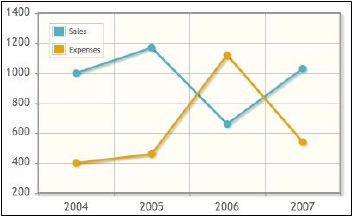
\includegraphics[scale=0.4]{img/obr3}
\end{figure}
\end{minipage}
\end{frame}


\begin{frame}[containsverbatim]\frametitle{RemoteCommand}
  \begin{itemize}
    \item RemoteCommand provides a simple way how to execute backing bean methods with JavaScript.
    \item[] \begin{footnotesize} \begin{verbatim}
<h:form>
    <p:remoteCommand name="rc" update="msgs" 
                     actionListener="#{remoteCommandView.execute}" />
    <p:growl id="msgs" showDetail="true" />
    <p:commandButton type="button" onclick="rc()" value="Execute" 
                     icon="ui-icon-refresh" />
</h:form>
\end{verbatim} \end{footnotesize}
     \item can be used also for partial processing of the form
     \item[] \begin{footnotesize} \begin{verbatim}
<h:form id="form">
    <p:remoteCommand name="updateList" update="users" process="@this" />
...
function handleMessage(message) {
    ...
    updateList();
}
\end{verbatim} \end{footnotesize}
  \end{itemize}
\begin{tikzpicture}[remember picture,overlay]
    \node[xshift=-0.6cm,yshift=-1.3cm] at (current page.north east){%
    
\includegraphics[width=1cm]{img/oko}};
\end{tikzpicture}
\end{frame}


\begin{frame}[containsverbatim]\frametitle{Push}
  \begin{itemize}
    \item Atmosphere framework is used for sending asynchronous messages from the server to the client.
	\item Requires special configuration (\texttt{web.xml})
	\item[] \begin{footnotesize} \begin{verbatim}
<servlet>
    <servlet-name>Push Servlet</servlet-name>
    <servlet-class>org.primefaces.push.PushServlet</servlet-class>
    <async-supported>true</async-supported>
</servlet>
<servlet-mapping>
    <servlet-name>Push Servlet</servlet-name>
    <url-pattern>/primepush/*</url-pattern>
</servlet-mapping>	
	\end{verbatim} \end{footnotesize}
    \item Uses annotations for defining push endpoints and message callbacks.
  \end{itemize}
\begin{tikzpicture}[remember picture,overlay]
    \node[xshift=-0.6cm,yshift=-1.3cm] at (current page.north east){%
    
\includegraphics[width=1cm]{img/naradi}};
\end{tikzpicture}
\end{frame}


\begin{frame}[containsverbatim]\frametitle{Push}
  \begin{itemize}
    \item \texttt{@PushEndpoint}
	  \begin{itemize}
		\item A class annotated with this annotation defines push channel, through which the server can contact the client.
	  \end{itemize}
    \item \texttt{@OnMessage}
	  \begin{itemize}
		\item When data are ready to be delivered, method annotated with this annotation will be called.
	  \end{itemize}
    \item Connection lifecycle annotations
      \begin{itemize}
    	\item \texttt{@OnOpen}
		\item \texttt{@OnClose}
      \end{itemize}
    \item \texttt{@PathParam}
      \begin{itemize}
    	\item parameters in path in URI
      \end{itemize}
    \item[] \begin{footnotesize} \begin{verbatim}
@PushEndpoint("/somepath/{room}/{user}")
@Singleton
public class ChatResource {
    @PathParam("room")
    private String room;
    @PathParam("user")
    private String username;
    ...
\end{verbatim} \end{footnotesize}
  \end{itemize}
\end{frame}


\begin{frame}[containsverbatim]\frametitle{Push}
  \begin{itemize}
    \item API
      \begin{itemize}
        \item \texttt{RemoteEndPoint}
          \begin{itemize}
            \item represents client-side browser
          \end{itemize}
    	\item \texttt{EventBus}
          \begin{itemize}
            \item class for interacting with Push endpoints
	        \item uses Pub-Sub and Point-to-Point messaging domains
            \item[] {\footnotesize \verb;EventBus eventBus =;}
            \item[] {\footnotesize \verb+    EventBusFactory.getDefault().eventBus();+}
            \item[] \verb+eventBus.publish("/counter", "Some data");+
          \end{itemize}
      \end{itemize}
	\item Encoders and decoders
      \begin{itemize}
    	\item has to be used when broadcasting a value
      \end{itemize}
    \item[] \begin{footnotesize} \begin{verbatim}
@PushEndpoint("/counter")
public class CounterResource {
    @OnMessage(encoders = {JSONEncoder.class})
    public String onMessage(String count) {
        return count;
    }
}
\end{verbatim} \end{footnotesize}
  \end{itemize}
\end{frame}

\begin{frame}[containsverbatim]\frametitle{Push}
  \begin{itemize}
    \item Client side
	  \begin{itemize}
		\item has to declare socket, through which it can accept the data.
        \item[] \begin{footnotesize} \begin{verbatim}
<h:form id="form">
    <h:outputText id="out" value="#{globalCounter.count}" />
    <p:commandButton value="Click" 
                     actionListener="#{globalCounter.increment}" />
</h:form>
 
<p:socket channel="/counter">
    <p:ajax event="message" update="form:out" />
</p:socket> 

\end{verbatim} \end{footnotesize}
        \item socket defines a channel
    	\item often convenient to use JavaScript
        \vspace{0.1cm}
        \item[] \begin{footnotesize} \begin{verbatim}
<p:socket onMessage="handleMessage" channel="/notify" />
<script type="text/javascript">
    function handleMessage(facesmessage) {
        facesmessage.severity = 'info';
        PF('growl').show([facesmessage]);
    }
</script>
\end{verbatim} \end{footnotesize}
      \end{itemize}
  \end{itemize}
\begin{textblock}{10}(9.7,0.2)
    {\footnotesize Example PFChat (JBoss)}
\end{textblock}
\end{frame}


\begin{frame}[fragile]\frametitle{RequestContext (PrimeFaces $<$ 7.0)}
  \begin{itemize}
    \item Update component(s) programmatically.
	  \begin{itemize}
		\item dynamic rendering
	  \end{itemize}
    \item Execute JavaScript from beans.
    \item[] \begin{footnotesize}
      \begin{verbatim}
if (!FacesContext.getCurrentInstance().isPostback()) {
  RequestContext.getCurrentInstance()
    .execute("alert('This onload script is added from backing bean.')");
}
\end{verbatim}
    \end{footnotesize}
 	\item Add AJAX callback parameters.
 	\item Scroll to a specific component after AJAX update.
  \end{itemize}
\end{frame}


\begin{frame}[fragile]\frametitle{Class PrimeFaces}
  \begin{itemize}
    \item Allows to update component(s) programmatically.
	  \begin{itemize}
		\item dynamic rendering
		\item \texttt{PrimeFaces.current().ajax().update()}
	  \end{itemize}
    \item Execute JavaScript from beans.
    \item[] \begin{footnotesize}
      \begin{verbatim}
if (!PrimeFacesContext.getCurrentInstance().isPostback()) {
  PrimeFaces.current()
  .executeScript("alert('This onload script is added from backing bean.')");
}
\end{verbatim}
    \end{footnotesize}
 	\item Add AJAX callback parameters.
 	\item Scroll to a specific component after AJAX update.
  \end{itemize}
\begin{textblock}{10}(9.5,3.6)
    {\footnotesize Example PFRequestContext}
\end{textblock}
\begin{tikzpicture}[remember picture,overlay]
    \node[xshift=-0.6cm,yshift=-1.3cm] at (current page.north east){%
    
\includegraphics[width=1cm]{img/lupa}};
\end{tikzpicture}
\end{frame}


\begin{frame}\frametitle{References}
  \begin{itemize}
    \item \url{http://www.primefaces.org/showcase/}
	\item \url{http://primefaces.org/}
    \item \url{http://www.ocpsoft.org/prettyfaces/}
    \item \url{http://blog.hatemalimam.com/using-prettyfaces-with-primefaces-upload/}
    \item \url{https://jqueryui.com/themeroller/}
  \end{itemize}
\end{frame}

\begin{frame}\frametitle{References}
  \begin{itemize}
    \item \url{https://github.com/primefaces/primefaces/tree/master/primefaces-showcase/src/main/java/org/primefaces/showcase/service}
    \item \url{https://primefaces.github.io/primefaces/10_0_0/\#/../migrationguide/migrationguide}
    \item \url{https://www.primefaces.org/showcase-ext/views/home.jsf}
    \item \url{https://github.com/primefaces-extensions/primefaces-extensions}
    \item \url{https://stackoverflow.com/questions/15146052/what-does-the-arrow-operator-do-in-java}
    \item \url{https://dzone.com/articles/java-8-lambda-functions-usage-examples}
    \item \url{https://showcase.omnifaces.org/push/socket}
    \item \url{https://stackoverflow.com/questions/30128395/identifying-and-solving-javax-el-propertynotfoundexception-target-unreachable}
  \end{itemize}
\end{frame}

\bluepage{Thank you for your attention!}



\end{document}
